\documentclass[../../main.tex]{subfiles}
\begin{document}

{\bf [解答]}

$4$の目が出る確率を
\begin{align}
  r = 1 - p - 4q \label{eq:1}
\end{align}
とする．各目が出る確率をまとめると下の表のようになる．

\begin{table}[htb]
  \centering
  \caption{カードの位置と対応する確率変数}
  \begin{tabular}{|c|c|c|c|c|c|}
    \hline
    1 & 2 & 3 & 4 & 5 & 6 \\ \hline
    $q$ & $q$ & $p$ & $r$ & $q$ & $q$ \\ \hline
  \end{tabular}
\end{table}

\paragraph{(1)}

\subparagraph{$1^{\circ}: a+b\le 4$となる事象$A$}

$a$としてとりうる値は$a=1,2,3$の三通りで，
それぞれ対応する$b$は$3$以下，$2$以下，$1$以下だから
求める確率は
\begin{align}
  P(A)
  &= q(q+q+p) + q(q+q) + pq = 4q^2 + 2pq \label{eq:2}
\end{align}
である．

\subparagraph{$2^{\circ}: a<b$となる事象$B$}

$1$と同様に$a$としてとりうる値 ($a=1,2,3,4,5$)で場合分けして考えると
求める確率は
\begin{align}
  P(B)
  &= q(1-q) + q(1-2q) + p(1-2q-p) + r(q+q) + q \cdot q \\
  &= -p^2 + p - 4pq - 10q^2 + 4q \quad (\because \text{\cref{eq:1}}) \label{eq:3}
\end{align}
である．
\casesend

\cref{eq:2,eq:3}を足し合わせて
\begin{align}
  E
  &= P(A) + P(B) \\
  &= 2(4q^2 + 2pq) + (-p^2 + p - 4pq - 10q^2 + 4q) \\
  &= -p^2 + p - 2q^2 + 4q \label{eq:4}
\end{align}
である．

\paragraph{(2)}

$\dfrac{1}{p} = n, \dfrac{1}{q} = m \; (n,m \in \mathbb{N})$ とおく．$0 < p, q, r < 1$ から，
\begin{align}
  0 < \dfrac{1}{n}, \dfrac{1}{m} < 1, \quad 0 < 1 - \dfrac{1}{n} - \dfrac{4}{m} < 1
\end{align}
前者から，
\begin{align}
  n, m \ge 2 \label{eq:5}
\end{align}
であり，後者から
\begin{align}
  0 < 4n + m < mn \label{eq:6}
\end{align}
である．\cref{eq:5}から左側の不等号の成立は明らかで，右側の不等号について考えると
\begin{align}
  (n-1)(m-4) > 4 \label{eq:7}
\end{align}
である．
以上\cref{eq:5,eq:7}を満たす自然数$n,m$の組は以下の表のようになる．

\begin{table}[htb]
  \centering
  \caption{\cref{eq:5,eq:7} をみたす $(n,m)$ の範囲}
  \begin{tabular}{c|c}
    $n$ & $m$ \\ \hline
    2 & $m \ge 9$ \\ \hline
    3 & $m \ge 7$ \\ \hline
    4 & $m \ge 6$ \\ \hline
    5 & $m \ge 6$ \\ \hline
    $n \ge 6$ & $m \ge 5$
  \end{tabular}
\end{table}

次に\cref{eq:4}を$m,n$で書き直すと
\begin{align}
  E
  &= -\Bigl(p - \dfrac{1}{2}\Bigr)^2 + \dfrac{1}{4} - 2(q-1)^2 + 2 \\
  &= \dfrac{9}{4} - \Bigl(\dfrac{2-n}{2n}\Bigr)^2 - 2\Bigl(\dfrac{1-m}{m}\Bigr)^2 \label{eq:8}
\end{align}
である．
第二項，第三項に対応する連続化した関数$y = f(x) = \dfrac{2-x}{2x}$， $y = g(x) = \dfrac{1-x}{x}$ を用いて
\begin{align}
  E = \dfrac{9}{4} - \left\{f(x)\right\}^2 - 2\left\{g(x)\right\}^2 \label{eq:9}
\end{align}
とかけ，$y=f(x),y=g(x)$のグラフは下図のようになる．

\begin{figure}[htb]
  \centering
  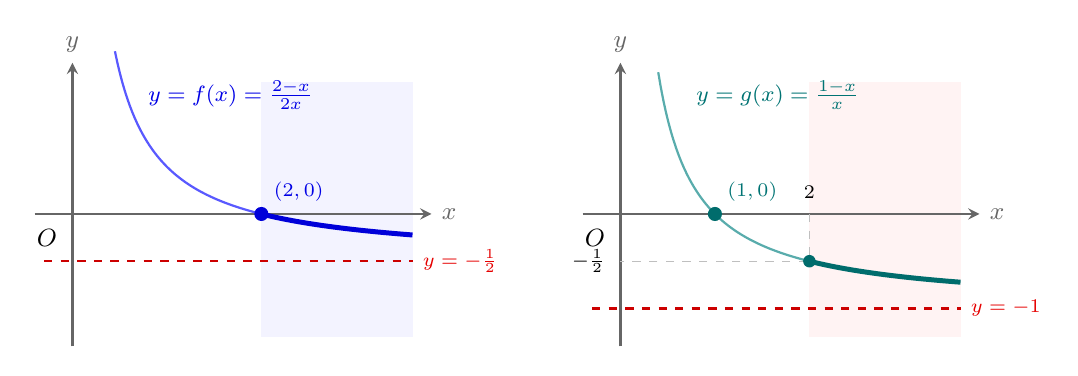
\begin{tikzpicture}[scale=1.2, >=stealth, every node/.style={font=\small}]

    % ============================================================
    % 【左側】y = f(x) = (2 - x) / (2x) = 1/x - 1/2
    % ============================================================
    \begin{scope}[xshift=0cm]
      % 注目区間 x >= 2 の背景ハイライト
      \fill[blue!6, opacity=0.8] (2.0, -1.3) rectangle (3.6, 1.4);

      % 水平漸近線 y = -1/2
      \draw[dashed, red!80!black, thick] (-0.3, -0.5) -- (3.6, -0.5)
      node[right, font=\scriptsize, red!90!black] {$y = -\frac{1}{2}$};

      % 座標軸
      \draw[->, thick, gray!80!black] (-0.4, 0) -- (3.8, 0) node[right] {$x$};
      \draw[->, thick, gray!80!black] (0, -1.4) -- (0, 1.6) node[above] {$y$};
      \node[below left=2pt] at (0, 0) {$O$};

      % 曲線 y = f(x)
      % (i) 0.5 <= x <= 2 (正から 0 へ)
      \draw[thick, blue!65, domain=0.45:2.0, samples=60]
      plot (\x, {(2.0 - \x)/(2.0*\x)});
      % (ii) x >= 2 (考察対象: 負で単調減少、太線強調)
      \draw[line width=1.8pt, blue!85!black, domain=2.0:3.6, samples=50]
      plot (\x, {(2.0 - \x)/(2.0*\x)});

      % x 切片 (2, 0)
      \node[circle, fill=blue!85!black, inner sep=1.8pt] at (2.0, 0) {};
      \node[above right=1pt, font=\scriptsize, blue!90!black] at (2.0, 0) {$(2, 0)$};

      % 曲線ラベル
      \node[blue!90!black, font=\footnotesize\bfseries, above right] at (0.7, 1.0)
      {$y = f(x) = \frac{2-x}{2x}$};

    \end{scope}

    % ============================================================
    % 【右側】y = g(x) = (1 - x) / x = 1/x - 1
    % ============================================================
    \begin{scope}[xshift=5.8cm]
      % 注目区間 x >= 2 の背景ハイライト
      \fill[red!6, opacity=0.8] (2.0, -1.3) rectangle (3.6, 1.4);

      % 水平漸近線 y = -1
      \draw[dashed, red!80!black, thick] (-0.3, -1.0) -- (3.6, -1.0)
      node[right, font=\scriptsize, red!90!black] {$y = -1$};

      % 座標軸
      \draw[->, thick, gray!80!black] (-0.4, 0) -- (3.8, 0) node[right] {$x$};
      \draw[->, thick, gray!80!black] (0, -1.4) -- (0, 1.6) node[above] {$y$};
      \node[below left=2pt] at (0, 0) {$O$};

      % 曲線 y = g(x)
      % (i) 0.4 <= x <= 2
      \draw[thick, teal!65, domain=0.4:2.0, samples=60]
      plot (\x, {(1.0 - \x)/\x});
      % (ii) x >= 2 (考察対象: 負で単調減少、太線強調)
      \draw[line width=1.8pt, teal!85!black, domain=2.0:3.6, samples=50]
      plot (\x, {(1.0 - \x)/\x});

      % x 切片 (1, 0)
      \node[circle, fill=teal!85!black, inner sep=1.8pt] at (1.0, 0) {};
      \node[above right=1pt, font=\scriptsize, teal!90!black] at (1.0, 0) {$(1, 0)$};

      % x = 2 での値 (2, -1/2)
      \draw[dashed, gray!50] (2.0, 0) -- (2.0, -0.5) -- (0, -0.5);
      \node[circle, fill=teal!85!black, inner sep=1.6pt] at (2.0, -0.5) {};
      \node[above=2pt, font=\scriptsize] at (2.0, 0) {$2$};
      \node[left=2pt, font=\scriptsize] at (0, -0.5) {$-\frac{1}{2}$};

      % 曲線ラベル
      \node[teal!90!black, font=\footnotesize\bfseries, above right] at (0.7, 1.0)
      {$y = g(x) = \frac{1-x}{x}$};

    \end{scope}

  \end{tikzpicture}
  \caption{$y=f(x)=\dfrac{2-x}{2x}$ と $y=g(x)=\dfrac{1-x}{x}$ のグラフ}
  \label{fig:hyperbolic_functions_fx_gx}
\end{figure}

さて，$2\le x$では$f(x)$も$g(x)$も負で単調減少だから，$\{f(x)\}^2,\{g(x)\}^2$は単調増加である．従って $E$ を最大にする候補は上表の等号成立時の $(n,m)$ である．また，$n=5$については明らかに$n=4$よりも$\{f(x)\}^2+2\{g(x)\}^2$が大きくなる（$m \ge 6$の条件が同じため）ので考えなくて良い．残りのケースについて具体的に$\{f(x)\}^2+2\{g(x)\}^2$を計算すると以下の表のようになる．

\begin{table}[htb]
  \centering
  \begin{tabular}{c|l}
    $(n,m)$ & $\{f(n)\}^2 + 2\{g(m)\}^2$ \\ \hline
    $(2,9)$ & $0 + 2\Bigl(\dfrac{8}{9}\Bigr)^2 = \dfrac{128}{81}$ \\ \hline
    $(3,7)$ & $\Bigl(\dfrac{1}{6}\Bigr)^2 + 2\Bigl(\dfrac{6}{7}\Bigr)^2 = \dfrac{7^2 + 2 \cdot 6^4}{6^2 \cdot 7^2}$ \\ \hline
    $(4,6)$ & $\Bigl(\dfrac{1}{4}\Bigr)^2 + 2\Bigl(\dfrac{5}{6}\Bigr)^2 = \dfrac{209}{9 \cdot 16}$ \\ \hline
    $(6,5)$ & $\Bigl(\dfrac{1}{3}\Bigr)^2 + 2\Bigl(\dfrac{4}{5}\Bigr)^2 = \dfrac{313}{9 \cdot 25}$
  \end{tabular}
  \caption{候補となる $(n,m)$ における $\{f(n)\}^2+2\{g(m)\}^2$ の値}
\end{table}

このうち$\{f(x)\}^2,\{g(x)\}^2$が最小になるのは$(n,m) = (6,5)$ の時で，この時 $E$ が最大である．よって求める $(p,q)$ は $(p,q) = \Bigl(\dfrac{1}{6}, \dfrac{1}{5}\Bigr)$ である．

\end{document}
